\chapter{Introduction to the dataset}
\label{app:A}
Appendices hold useful data which is not essential to understand the work
done in the master's thesis. An example is a (program) source.
An appendix can also have sections as well as figures and references\cite{h2g2}.

\section{More Lorem}

\begin{figure}[h!]
	\centering
	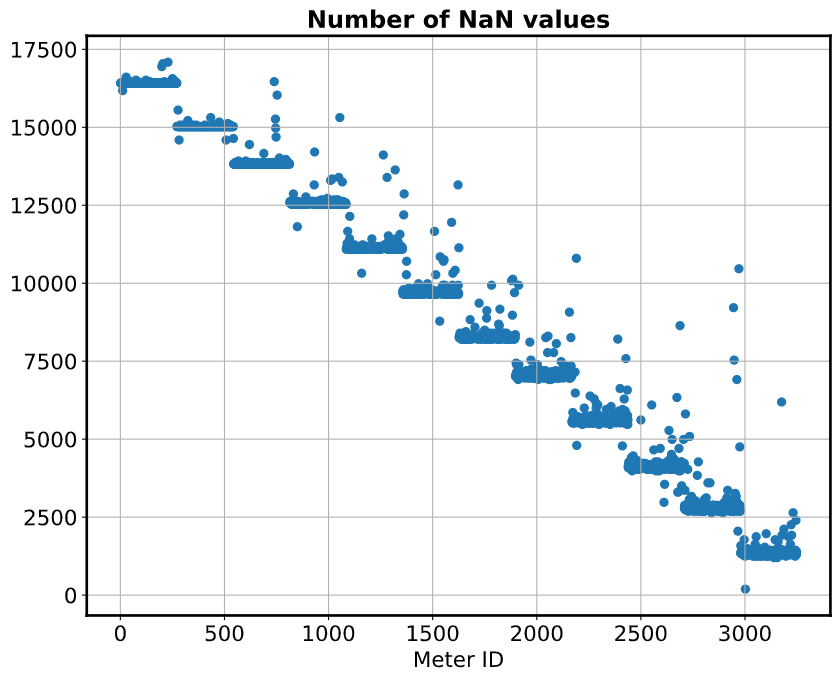
\includegraphics[width=0.8\textwidth]{amountNaN.png}
	\caption{The amount of NaN values in all the 3248 smart meters.}
	\label{fig:amountNaN}
\end{figure}
\subsection{Lorem 15--17}

\begin{table}[h]
	\centering
	\begin{tabular}{|p{5cm}|p{2.5cm}|}
		\hline
		\textbf{Attribute} & \textbf{Filled places}\\ \hline	
		Dwelling type  & 1702\\ \hline
		\# Occupants & 74\\ \hline
		Heating fuel & 1859\\ \hline
		Heating fuel & 78\\ \hline
		Hot water fuel & 76\\ \hline
		Boiler age & 74\\ \hline
		Loft insulation & 75\\ \hline
		Wall insulation & 75\\ \hline
		Heating temperature & 74\\ \hline
		Efficient lighting percentage & 73\\ \hline
		Dishwasher & 76\\ \hline
		Freezer & 70\\ \hline
		Fridge freezer & 70\\ \hline
		Refrigerator & 73\\ \hline
		Tumble Dryer & 76\\ \hline
		Washing machine & 76\\ \hline
		Game console &72\\ \hline
		Laptop & 70\\ \hline
		Pc & 70\\ \hline
		Router & 69\\ \hline
		Set top box & 70\\ \hline
		Tablet & 70\\ \hline
		Tv & 75\\ \hline
		
	\end{tabular}
	\caption{Amount of response on the voluntary questionnaires. }
	\label{tab:attributes}
\end{table}


\subsection{Lorem 18--19}


\section{Lorem 51}


%%% Local Variables: 
%%% mode: latex
%%% TeX-master: "thesis"
%%% End: 
